% ============================================================
% Software Requirements Specification (SRS)
% Platform PasarKita -- Marketplace Digital UMKM
% Kelompok 2 -- Rekayasa Perangkat Lunak 2
% ============================================================

\documentclass[12pt,a4paper]{article}

% ============================================================
% Packages
% ============================================================
\usepackage[utf8]{inputenc}
\usepackage[T1]{fontenc}
\usepackage[sfdefault]{carlito} % Calibri-compatible sans-serif font
\usepackage[scaled=0.85]{inconsolata} % Consolas clone for monospace
\usepackage{amsmath}
\usepackage[english,indonesian]{babel}
\usepackage{geometry}
\usepackage{setspace}
\usepackage{titlesec}
\usepackage{graphicx}
\usepackage{hyperref}
\usepackage{booktabs}
\usepackage{array}
\usepackage[format=hang,font=footnotesize,labelfont=bf]{caption}
\usepackage{enumitem}
\usepackage{parskip}
\usepackage{fancyhdr}
\usepackage{tocloft}
\usepackage{tabularx}
\usepackage{longtable}
\usepackage{ragged2e}
\usepackage{xcolor}
\usepackage{listings}
\usepackage{multirow}
\usepackage{etoolbox}   % Untuk AtBeginEnvironment

% ============================================================
% Page Setup -- margin diperlebar (teks lebih lebar)
% ============================================================
\geometry{
    top=3cm,
    bottom=2.5cm,
    left=2.5cm,
    right=2cm,
    headheight=20pt,
    headsep=15pt
}

% ============================================================
% Title Formatting -- tanpa BAB, rata kiri
% ============================================================
\titleformat{\section}
    {\normalfont\fontsize{14}{17}\bfseries\raggedright}{\thesection.}{0.5em}{}

\titleformat{\subsection}
    {\normalfont\fontsize{12}{14}\bfseries\raggedright}{\thesubsection}{1em}{}

\titleformat{\subsubsection}
    {\normalfont\fontsize{12}{14}\normalfont\raggedright}{\thesubsubsection}{1em}{}

\titlespacing*{\section}{0pt}{18pt}{6pt}
\titlespacing*{\subsection}{0pt}{12pt}{4pt}

% ============================================================
% Spacing
% ============================================================
\onehalfspacing

% ============================================================
% Header/Footer
% ============================================================
\definecolor{bannerblue}{RGB}{79, 129, 189}

\pagestyle{fancy}
\fancyhf{}

\fancyhead[C]{%
    \colorbox{bannerblue}{%
        \parbox{\dimexpr\textwidth-2\fboxsep\relax}{%
            \centering\color{white}\sffamily\fontsize{9}{10}\selectfont%
            \textbf{SRS -- PLATFORM PASARKITA (DOKUMEN REKAYASA 2026)}%
        }%
    }%
}

\fancyfoot[L]{\sffamily\fontsize{9}{10}\selectfont Kelompok 2 -- Rekayasa Perangkat Lunak 2}
\fancyfoot[R]{\sffamily\fontsize{9}{10}\selectfont\thepage}
\renewcommand{\headrulewidth}{0pt}

% ============================================================
% Hyperref
% ============================================================
\hypersetup{
    colorlinks=true,
    linkcolor=black,
    citecolor=black,
    filecolor=black,
    urlcolor=black,
    pdftitle={SRS Platform PasarKita},
    pdfauthor={Kelompok 2 RPL 2},
    pdfsubject={Software Requirements Specification},
}

% ============================================================
% Table of Contents Customization
% ============================================================
\renewcommand{\contentsname}{DAFTAR ISI}
\renewcommand{\cfttoctitlefont}{\hfill\fontsize{14}{17}\selectfont\bfseries}
\renewcommand{\cftaftertoctitle}{\hfill}

\renewcommand{\listtablename}{DAFTAR TABEL}
\renewcommand{\cftlottitlefont}{\hfill\fontsize{14}{17}\selectfont\bfseries}
\renewcommand{\cftafterlottitle}{\hfill}

\renewcommand{\listfigurename}{DAFTAR GAMBAR}
\renewcommand{\cftloftitlefont}{\hfill\fontsize{14}{17}\selectfont\bfseries}
\renewcommand{\cftafterloftitle}{\hfill}

% ============================================================
% Subsection Numbering
% ============================================================
\renewcommand{\thesubsection}{\arabic{section}.\arabic{subsection}}
\renewcommand{\thesubsubsection}{\arabic{section}.\arabic{subsection}.\arabic{subsubsection}}

% ============================================================
% Longtable -- font kecil otomatis di semua longtable
% ============================================================
\AtBeginEnvironment{longtable}{\footnotesize\setlength{\tabcolsep}{4pt}}

% ============================================================
% Listings Setup
% ============================================================
\definecolor{codebg}{RGB}{248,248,248}
\definecolor{codecomment}{RGB}{100,100,100}
\definecolor{codestring}{RGB}{163,21,21}

\lstset{
    backgroundcolor=\color{codebg},
    basicstyle=\ttfamily\footnotesize,
    commentstyle=\color{codecomment},
    stringstyle=\color{codestring},
    breaklines=true,
    breakatwhitespace=true,
    frame=single,
    framesep=3pt,
    rulecolor=\color{gray},
    xleftmargin=10pt,
    xrightmargin=10pt,
    captionpos=b,
    numbers=none,
    showstringspaces=false,
    tabsize=2,
}

% ============================================================
% Column Type untuk Longtable (rata kiri)
% ============================================================
\newcolumntype{L}[1]{>{\RaggedRight\arraybackslash\footnotesize\setlength{\parindent}{0pt}\emergencystretch=1.5em}p{#1}}

% ============================================================
% Beginning of Document
% ============================================================
\begin{document}

\renewcommand{\contentsname}{DAFTAR ISI}
\renewcommand{\listtablename}{DAFTAR TABEL}
\renewcommand{\listfigurename}{DAFTAR GAMBAR}

\sffamily
\raggedright

% ============================================================
% Judul Dokumen (tanpa halaman cover terpisah)
% ============================================================
\begin{flushleft}
    {\fontsize{18}{22}\selectfont\sffamily\textbf{SOFTWARE REQUIREMENTS SPECIFICATION}\par}
    \vspace{0.2cm}
    {\fontsize{14}{18}\selectfont\sffamily\textbf{Platform PasarKita}\par}
    {\fontsize{12}{14}\selectfont\sffamily\textit{Marketplace Digital UMKM}\par}
\end{flushleft}

\vspace{0.4cm}

\begin{longtable}{|L{4.0cm}|L{11.8cm}|}
    \hline
    \textbf{Atribut} & \textbf{Nilai} \\
    \hline
    Nama Dokumen & Software Requirements Specification (SRS) Platform PasarKita \\
    \hline
    Versi & 1.0 -- Initial Requirements Baseline \\
    \hline
    Tanggal & 24 Juni 2026 \\
    \hline
    Sistem & Marketplace PasarKita \\
    \hline
    Pemilik Produk & Kelompok 2 RPL 2 / Universitas Logistik dan Bisnis Internasional \\
    \hline
    Target Pembaca & Product owner, developer, QA engineer, maintainer, dan dosen pengampu \\
    \hline
    Status & Dokumen kerja untuk baseline requirement dan validasi implementasi \\
    \hline
    \multicolumn{2}{|L{16.2cm}|}{
        \textbf{Basis Penyusunan} \vspace{0.15cm} \newline
        SRS ini disusun dari kode dan konfigurasi aplikasi PasarKita yang aktif: frontend Next.js App Router (\path{frontend/}), backend REST API Express (\path{backend/src/}), skema database Supabase PostgreSQL (\path{backend/database/schema/000_full_schema.sql}), serta integrasi dengan SmartBank dan LogistiKita. Struktur dokumen mengikuti pola SRS yang lazim digunakan tim engineering: tujuan, scope, konteks sistem, aktor, constraint, kebutuhan spesifik, interface, data, business rules, risiko, acceptance criteria, dan traceability.
    } \\
    \hline
\end{longtable}

\clearpage

% ============================================================
% DAFTAR ISI
% ============================================================
\section*{Daftar Isi}
\phantomsection
\addcontentsline{toc}{section}{Daftar Isi}

\begin{longtable}{|L{2.5cm}|L{13.2cm}|}
    \hline
    \textbf{Bagian} & \textbf{Isi} \\
    \hline
    1 & Pendahuluan dan Konteks Dokumen \\
    \hline
    2 & Gambaran Produk dan Batas Sistem \\
    \hline
    3 & Konteks Operasional dan Arsitektur \\
    \hline
    4 & Domain Data dan Aturan Bisnis \\
    \hline
    5 & Kebutuhan Fungsional \\
    \hline
    6 & Kebutuhan Non-Fungsional \\
    \hline
    7 & Antarmuka Eksternal \\
    \hline
    8 & Workflow Operasional \\
    \hline
    9 & Risiko, Kontrol, dan Acceptance Criteria \\
    \hline
    10 & Matriks Ketertelusuran \\
    \hline
    Lampiran & Glosarium, Referensi Internal, dan Catatan Perubahan Versi \\
    \hline
\end{longtable}

\clearpage

% ============================================================
% BAB 1
% ============================================================
\setcounter{section}{0}

\section{Pendahuluan dan Konteks Dokumen}
% ============================================================
% BAB 1 - PENDAHULUAN DAN KONTEKS DOKUMEN
% ============================================================

\subsection{Tujuan Dokumen}

Dokumen ini mendefinisikan kebutuhan perangkat lunak untuk PasarKita sebagai
komponen \textit{Demand Generator} B2C dalam ekosistem \textit{microservices}
UMKM RPL 2.

SRS ini berfungsi sebagai \textit{baseline} bersama antara pemilik produk,
pengembang, penguji, dan pengelola sistem. Dokumen tidak dimaksudkan sebagai
uraian konseptual, melainkan sebagai spesifikasi yang menerjemahkan perilaku
aplikasi ke dalam kebutuhan yang dapat dibangun, diuji, dan dipelihara. Setiap
kebutuhan dirumuskan agar memiliki ruang lingkup yang jelas, dasar implementasi
yang dapat ditelusuri, dan kriteria penerimaan yang dapat diverifikasi.

Rujukan format yang digunakan adalah praktik SRS yang umum dipakai di lingkungan
pengembangan perangkat lunak: dokumen dimulai dari tujuan dan \textit{scope},
dilanjutkan dengan \textit{product perspective}, \textit{user classes},
\textit{constraints}, asumsi, kebutuhan fungsional, kebutuhan non-fungsional,
\textit{external interfaces}, \textit{data requirements}, \textit{business rules},
\textit{acceptance criteria}, dan \textit{traceability matrix}. Dengan struktur
tersebut, dokumen dapat dipakai sebagai kontrak kerja teknis tanpa bergantung
pada penjelasan lisan.

% ----
\subsection{Ruang Lingkup Produk}

PasarKita adalah platform \textit{marketplace} digital B2C yang memfasilitasi
transaksi produk UMKM antara \textit{seller} dan \textit{buyer}. Sistem berjalan
sebagai aplikasi web \textit{fullstack} dengan \textit{frontend} Next.js 16.2
(di-\textit{deploy} ke \texttt{pasarkita.vercel.app}) dan \textit{backend}
Express.js berbasis \textit{serverless} (di-\textit{deploy} ke
\texttt{pasarkita-api.vercel.app}), menggunakan Supabase PostgreSQL sebagai
\textit{database}.

Dalam arsitektur ekosistem, PasarKita berperan sebagai \textbf{Demand
Generator}---inisiator transaksi di sisi permintaan. Semua transaksi keuangan
diproses oleh SmartBank (Kelompok 1), semua komunikasi antar-\textit{service}
melewati API Gateway (Kelompok 7), dan pengiriman dikoordinasikan oleh LogistiKita
(Kelompok 5). PasarKita tidak mengambil alih fungsi pembayaran, \textit{routing},
atau logistik dari \textit{service partner} tersebut.

Sistem PasarKita bertanggung jawab pada siklus transaksi \textit{marketplace}:
registrasi/autentikasi \textit{user}, pengelolaan katalog produk UMKM, keranjang
belanja, proses \textit{checkout} dengan kalkulasi \textit{fee}, koordinasi
pembayaran ke SmartBank, \textit{trigger} pengiriman ke LogistiKita, manajemen
status \textit{order}, dan \textit{dashboard analytics} untuk \textit{superadmin}.

% ----
\subsection{Out of Scope}

Dokumen ini tidak menspesifikasikan logika pembayaran internal SmartBank,
mekanisme \textit{routing} JWT API Gateway, algoritma penentuan tarif pengiriman
LogistiKita, ataupun manajemen akun dari \textit{service partner} lain.

\begin{longtable}{|L{3.5cm}|L{3cm}|L{8.5cm}|}
    \caption{Area di Luar dan di Dalam Lingkup SRS}
    \label{tab:scope} \\
    \hline
    \textbf{Area} & \textbf{Status Scope} & \textbf{Rasional} \\
    \hline
    \endfirsthead
    \hline
    \textbf{Area} & \textbf{Status Scope} & \textbf{Rasional} \\
    \hline
    \endhead
    \hline
    \endfoot
    Pemrosesan pembayaran
        & Di luar \textit{scope}
        & Seluruh transaksi keuangan diproses SmartBank melalui API Gateway.
          PasarKita hanya mengirim \textit{payment request} dan membaca \textit{response}. \\
    \hline
    \textit{Routing} dan JWT validation (inter-service)
        & Di luar \textit{scope}
        & API Gateway (Kelompok 7) bertanggung jawab atas \textit{routing}, JWT
          \textit{issuance} antar-\textit{service}, dan \textit{logging}
          inter-\textit{service}. \\
    \hline
    Kalkulasi tarif dan \textit{tracking} pengiriman internal
        & Di luar \textit{scope}
        & LogistiKita (Kelompok 5) mengelola logika pengiriman. PasarKita hanya
          men-\textit{trigger} dan membaca \texttt{tracking\_id}. \\
    \hline
    Manajemen stok \textit{supplier}
        & Di luar \textit{scope}
        & SupplierHub (Kelompok 4) mengelola \textit{supply chain}. PasarKita
          hanya membaca stok lokal dari \textit{database} sendiri. \\
    \hline
    Laporan keuangan konsolidasi ekosistem
        & Di luar \textit{scope}
        & UMKM Insight (Kelompok 6) mengonsumsi \textit{ledger} dari SmartBank.
          PasarKita hanya menyediakan data transaksi lokal via \textit{analytics endpoint}. \\
    \hline
    Manajemen produk CRUD \textit{seller} (WarungPOS)
        & Di luar \textit{scope}
        & WarungPOS (Kelompok 3) memiliki katalog tersendiri. PasarKita mengelola
          katalog produk \textit{seller} yang terdaftar di platformnya sendiri. \\
    \hline
    Manajemen saldo dompet \textit{user}
        & Di dalam \textit{scope} (partial)
        & PasarKita menyimpan \textit{snapshot} saldo lokal dari SmartBank untuk
          keperluan validasi awal, namun \textit{authoritative balance} tetap di SmartBank. \\
    \hline
    Katalog produk, \textit{order}, dan ulasan
        & Di dalam \textit{scope}
        & PasarKita adalah \textit{system of record} untuk produk, \textit{order},
          \texttt{order\_items}, dan \textit{ratings} dalam ekosistemnya. \\
    \hline
\end{longtable}

\clearpage

% ============================================================
% BAB 2
% ============================================================
\section{Gambaran Produk dan Batas Sistem}
% ============================================================
% BAB 2 - GAMBARAN PRODUK DAN BATAS SISTEM
% ============================================================

\subsection{Product Perspective}

Aplikasi ini menempati posisi sebagai \textbf{Demand Generator B2C} dalam
ekosistem \textit{microservices} UMKM RPL 2. Secara teknis, \textit{frontend}
berjalan di \texttt{pasarkita.vercel.app} (Next.js 16.2) dan \textit{backend}
di \texttt{pasarkita-api.vercel.app} (Express.js \textit{serverless}), keduanya
di-\textit{deploy} terpisah dari repo monorepo yang sama. \textit{Database}
menggunakan Supabase PostgreSQL yang diakses eksklusif oleh \textit{backend}
PasarKita.

Semua komunikasi ke \textit{service} eksternal (SmartBank, LogistiKita) melewati
API Gateway (Kelompok 7) dengan JWT. Untuk keperluan \textit{development} lokal,
tersedia \textit{mock server} di direktori \texttt{mock/} yang mensimulasikan
SmartBank (:4001) dan LogistiKita (:4002).

% Placeholder diagram konteks
\begin{figure}[htbp]
    \centering
    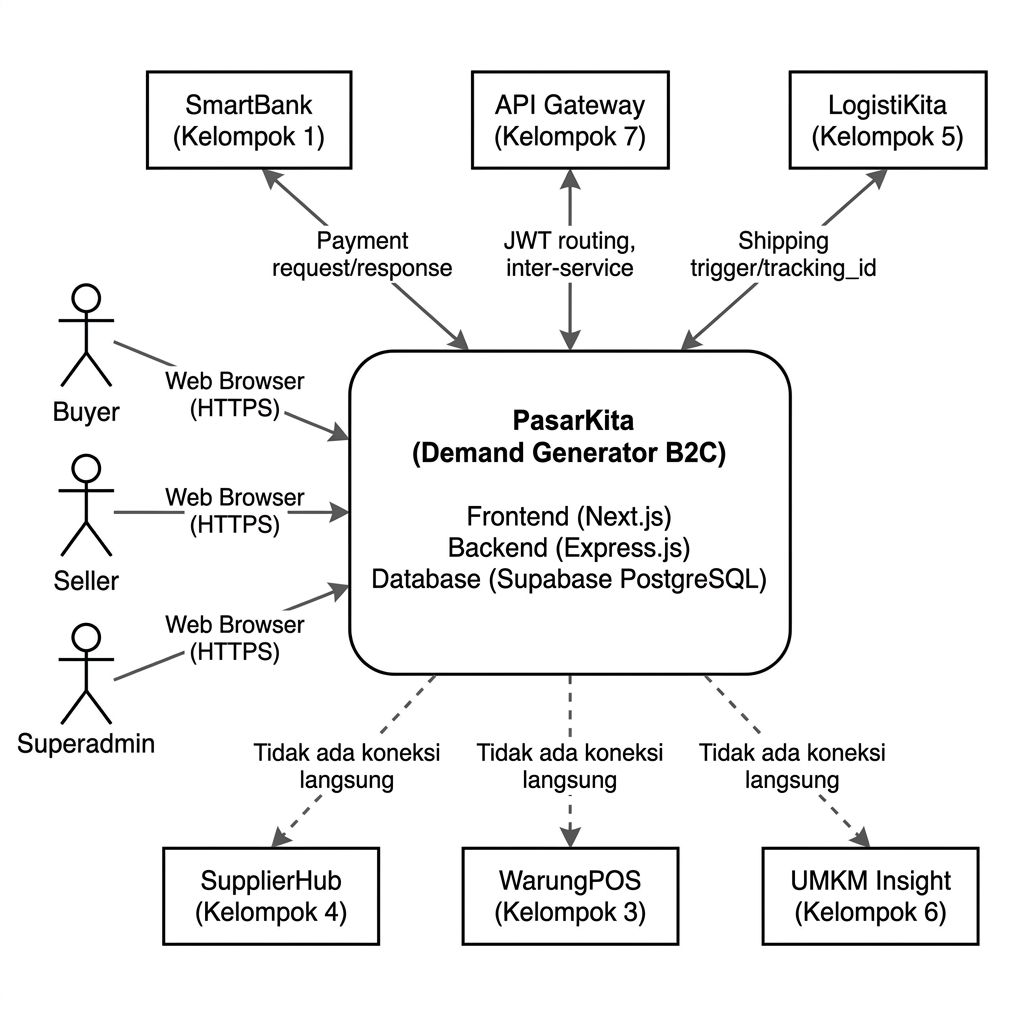
\includegraphics[width=\textwidth]{figures/diagram-konteks.png}
    \caption{Diagram Konteks Sistem PasarKita dalam Ekosistem UMKM RPL 2}
    \label{fig:diagram-konteks}
\end{figure}

% ----
\subsection{User Classes dan Karakteristik}

Sistem melayani beberapa kelas pengguna dengan hak dan ekspektasi yang berbeda.
Kebutuhan sistem harus menjaga perbedaan tersebut agar transaksi
\textit{marketplace} dapat berjalan tanpa mencampuri domain \textit{service} lain
dalam ekosistem.

\begin{longtable}{|L{2.2cm}|L{3.8cm}|L{4.5cm}|L{4cm}|}
    \caption{User Classes dan Karakteristik}
    \label{tab:user-classes} \\
    \hline
    \textbf{User Class} & \textbf{Tanggung Jawab} & \textbf{Ekspektasi Sistem}
        & \textbf{Kontrol Akses} \\
    \hline
    \endfirsthead
    \hline
    \textbf{User Class} & \textbf{Tanggung Jawab} & \textbf{Ekspektasi Sistem}
        & \textbf{Kontrol Akses} \\
    \hline
    \endhead
    \hline
    \endfoot
    Buyer
        & Menelusuri produk, menambahkan ke keranjang, melakukan \textit{checkout},
          memantau status \textit{order}, dan memberikan ulasan.
        & Alur belanja yang mudah, status \textit{order} \textit{real-time},
          konfirmasi pembayaran jelas, riwayat pesanan tersedia.
        & JWT role \texttt{buyer}; tidak dapat mengelola produk atau melihat \textit{analytics}. \\
    \hline
    Seller
        & Mengelola katalog produk sendiri (CRUD), memantau \textit{order} masuk,
          mengelola stok, dan membalas ulasan.
        & \textit{Dashboard} produk yang efisien, notifikasi \textit{order} baru,
          visibilitas stok rendah.
        & JWT role \texttt{seller}; hanya dapat CRUD produk milik sendiri; tidak
          dapat mengakses data \textit{seller} lain. \\
    \hline
    Superadmin
        & Memantau seluruh operasional platform: manajemen \textit{user},
          \textit{order}, \textit{analytics}, moderasi konten, dan \textit{audit log}.
        & \textit{Dashboard analytics} lengkap, kemampuan ban/aktifkan \textit{user},
          \textit{update} status \textit{order} manual, akses \textit{audit log}.
        & JWT role \texttt{superadmin}; dibuat via \textit{insert} manual ke
          Supabase; akses penuh ke semua \textit{endpoint} admin. \\
    \hline
    API Gateway
        & Memvalidasi JWT antar-\textit{service}, meneruskan \textit{payment request}
          ke SmartBank, dan \textit{trigger} ke LogistiKita.
        & Kontrak JSON stabil, \textit{error response} deterministik,
          \textit{idempotency key} pada \textit{checkout}.
        & \textit{Service-to-service} via \textit{header} JWT ekosistem; bukan
          \textit{user} biasa. \\
    \hline
    SmartBank
        & Memproses pembayaran dan mengembalikan \texttt{transaction\_id} atau
          \textit{failure response}.
        & Format \textit{request} konsisten, \textit{idempotency} terjaga,
          \textit{rollback} stok saat pembayaran gagal.
        & Akses melalui API Gateway; tidak ada akses langsung ke \textit{database}
          PasarKita. \\
    \hline
\end{longtable}

% ----
\subsection{Operating Environment}

\begin{longtable}{|L{2.8cm}|L{5.5cm}|L{6.2cm}|}
    \caption{Operating Environment Sistem PasarKita}
    \label{tab:operating-env} \\
    \hline
    \textbf{Komponen} & \textbf{Spesifikasi Saat Ini} & \textbf{Implikasi Requirement} \\
    \hline
    \endfirsthead
    \hline
    \textbf{Komponen} & \textbf{Spesifikasi Saat Ini} & \textbf{Implikasi Requirement} \\
    \hline
    \endhead
    \hline
    \endfoot
    Frontend
        & Next.js 16.2, App Router, TypeScript, Tailwind CSS, shadcn/ui,
          di-\textit{deploy} ke Vercel (\texttt{frontend/}).
        & \textit{Routing} berbasis App Router; komponen UI harus konsisten dengan
          shadcn/ui \textit{design system}. \\
    \hline
    Backend
        & Express.js dengan \texttt{serverless-http}, di-\textit{deploy} ke Vercel
          \textit{serverless function} (\texttt{backend/api/index.js}).
        & Tidak ada \textit{persistent in-memory state}; semua \textit{state} harus
          tersimpan di \textit{database}. \\
    \hline
    Database
        & Supabase PostgreSQL, diakses via Supabase SDK dan \textit{service role key}
          dari \textit{backend}.
        & Skema harus menjaga \texttt{users}, \texttt{products}, \texttt{orders},
          \texttt{order\_items}, \texttt{ratings}, \texttt{notifications},
          \texttt{vouchers}, dan \texttt{audit logs}. \\
    \hline
    State Management
        & Zustand (auth, cart) dan TanStack Query di \textit{frontend}.
        & \textit{Cart state} bersifat \textit{client-side}; sinkronisasi stok
          terjadi saat \textit{checkout} di \textit{backend}. \\
    \hline
    Auth
        & JWT yang di-\textit{generate} \textit{backend} PasarKita saat \textit{login};
          validasi JWT antar-\textit{service} via API Gateway.
        & Token harus menyertakan \textit{role}; \textit{middleware} auth harus
          memvalidasi sebelum setiap \textit{protected route}. \\
    \hline
    Integrasi Ekosistem
        & API Gateway di \texttt{GATEWAY\_BASE\_URL}; SmartBank dan LogistiKita
          diakses via Gateway.
        & Koneksi eksternal harus gagal secara terkendali dan tidak merusak data
          \textit{order} lokal. \\
    \hline
    Mock Server (dev)
        & Express.js lokal di \texttt{mock/smartbank/:4001} dan
          \texttt{mock/logistikita/:4002}.
        & Hanya digunakan saat \texttt{NODE\_ENV=development}; \textit{production}
          selalu melalui \texttt{GATEWAY\_BASE\_URL}. \\
    \hline
    Deploy
        & Dua project Vercel terpisah dari satu repo monorepo (\texttt{frontend/}
          dan \texttt{backend/}).
        & \textit{Environment variables} harus dikonfigurasi terpisah per project
          di Vercel. \\
    \hline
\end{longtable}

\clearpage

% ============================================================
% BAB 3
% ============================================================
\section{Konteks Operasional dan Arsitektur}
% ============================================================
% BAB 3 - KONTEKS OPERASIONAL DAN ARSITEKTUR
% ============================================================

\subsection{Architectural Overview}

Aplikasi menggunakan arsitektur \textbf{monorepo dua-tier} dengan pemisahan
\textit{frontend} dan \textit{backend} yang di-\textit{deploy} secara independen.
\textit{Backend} menggunakan pola modular berbasis domain (\texttt{src/modules/})
dengan \textit{middleware} terpusat untuk auth, validasi, dan \textit{error
handling}. \textit{Frontend} menggunakan App Router Next.js dengan komponen
shadcn/ui dan \textit{state management} Zustand.

\begin{longtable}{|L{3.5cm}|L{5cm}|L{6.5cm}|}
    \caption{Lapisan Arsitektur Sistem PasarKita}
    \label{tab:arsitektur} \\
    \hline
    \textbf{Lapisan} & \textbf{Artefak Utama} & \textbf{Tanggung Jawab} \\
    \hline
    \endfirsthead
    \hline
    \textbf{Lapisan} & \textbf{Artefak Utama} & \textbf{Tanggung Jawab} \\
    \hline
    \endhead
    \hline
    \endfoot
    Frontend: Routing
        & \texttt{frontend/app/} (App Router)
        & Mengarahkan halaman ke komponen React berdasarkan URL. \\
    \hline
    Frontend: UI Components
        & \texttt{frontend/components/}
        & Menyajikan halaman \textit{buyer} (katalog, \textit{cart},
          \textit{checkout}, \textit{order}), \textit{seller}
          (\textit{dashboard}, CRUD produk), dan admin
          (\textit{analytics}, manajemen \textit{user}). \\
    \hline
    Frontend: State
        & \texttt{frontend/store/} (Zustand)
        & Mengelola auth \textit{state} (\textit{user}, token) dan \textit{cart
          state} (\textit{items}, \textit{quantity}) secara \textit{client-side}. \\
    \hline
    Frontend: API Client
        & \texttt{frontend/lib/}
        & \textit{Wrapper} Axios/fetch ke \textit{backend} API dengan \textit{token
          injection} dari Zustand auth \textit{store}. \\
    \hline
    Backend: Entry Point
        & \texttt{backend/api/index.js}
        & \textit{Serverless entry point}; \textit{mounting} semua \textit{router}
          Express. \\
    \hline
    Backend: Modules
        & \texttt{backend/src/modules/} (auth, products, orders, checkout,
          integrations)
        & \textit{Business logic} per domain: autentikasi, katalog produk,
          manajemen \textit{order}, alur \textit{checkout}, dan komunikasi ke
          \textit{service} eksternal. \\
    \hline
    Backend: Middlewares
        & \texttt{backend/src/middlewares/} (auth, validate, errorHandler)
        & Validasi JWT, validasi Zod \textit{schema request body}, dan
          \textit{centralized error response}. \\
    \hline
    Backend: Integrations
        & \texttt{backend/src/integrations/} (smartbank, logistikita)
        & Adapter HTTP untuk komunikasi ke SmartBank dan LogistiKita via API
          Gateway. \\
    \hline
    Backend: Utils
        & \texttt{backend/src/utils/} (fee, response)
        & Kalkulasi \textit{fee marketplace} (2\%), \textit{helper} format
          \textit{response} JSON standar. \\
    \hline
    Database
        & Supabase PostgreSQL
        & Penyimpanan persisten untuk semua entitas domain PasarKita. \\
    \hline
\end{longtable}

% ----
\subsection{Data Flow}

Alur utama dimulai dari registrasi atau \textit{login} \textit{user} di
\textit{frontend}. Setelah autentikasi, \textit{buyer} menelusuri produk,
menambahkan ke \textit{cart} (\textit{state} Zustand), dan melakukan
\textit{checkout}. Saat \textit{checkout}, \textit{backend} memvalidasi stok,
menghitung total + \textit{fee} 2\%, membuat \textit{order} dengan status
\texttt{pending}, lalu mengirim \textit{payment request} ke SmartBank via API
Gateway.

\begin{figure}[htbp]
    \centering
    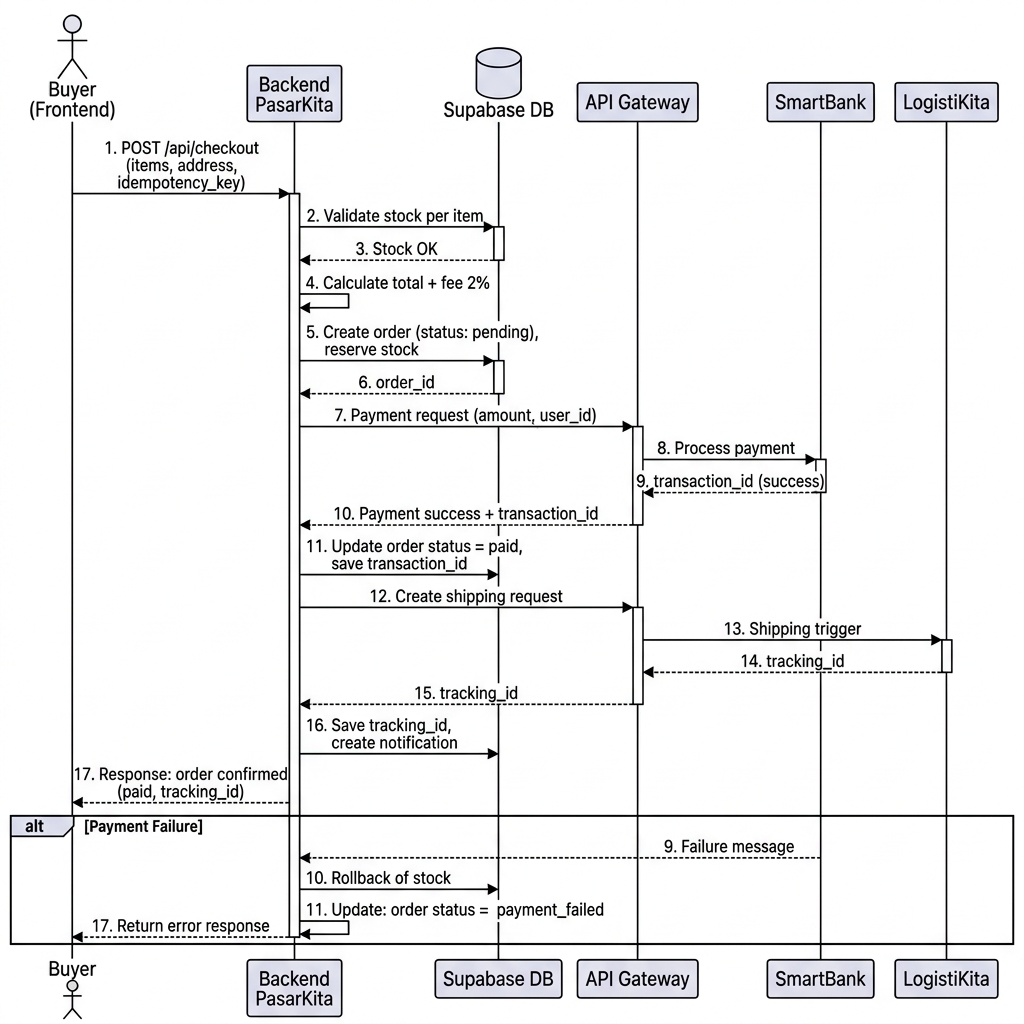
\includegraphics[width=\textwidth]{figures/sequence-checkout.png}
    \caption{Sequence Diagram Alur Checkout PasarKita}
    \label{fig:sequence-checkout}
\end{figure}

Jika pembayaran sukses, \textit{backend} memperbarui \textit{order} ke status
\texttt{paid}, mengirim \textit{trigger} pengiriman ke LogistiKita, menerima
\texttt{tracking\_id}, dan mencatat notifikasi. Jika gagal, stok di-\textit{rollback}
dan \textit{order} diperbarui ke \texttt{payment\_failed}. \textit{Superadmin}
dapat memantau seluruh alur melalui \textit{analytics endpoint} dan
\textit{audit log}.

\clearpage

% ============================================================
% BAB 4
% ============================================================
\section{Domain Data dan Aturan Bisnis}
% ============================================================
% BAB 4 - DOMAIN DATA DAN ATURAN BISNIS
% ============================================================

\subsection{Core Domain Entities}

\begin{longtable}{|L{2.8cm}|L{3cm}|L{4.7cm}|L{4cm}|}
    \caption{Core Domain Entities PasarKita}
    \label{tab:domain-entities} \\
    \hline
    \textbf{Entitas} & \textbf{Deskripsi} & \textbf{Field Penting}
        & \textbf{Catatan Ownership} \\
    \hline
    \endfirsthead
    \hline
    \textbf{Entitas} & \textbf{Deskripsi} & \textbf{Field Penting}
        & \textbf{Catatan Ownership} \\
    \hline
    \endhead
    \hline
    \endfoot
    \texttt{users}
        & Akun \textit{buyer}, \textit{seller}, dan \textit{superadmin}.
        & \texttt{id}, \texttt{name}, \texttt{email}, \texttt{password\_hash},
          \texttt{role}, \texttt{is\_active}, \texttt{phone}, \texttt{avatar\_url}
        & PasarKita adalah \textit{system of record} untuk akun \textit{user}
          dalam ekosistemnya. Saldo dikelola SmartBank. \\
    \hline
    \texttt{seller\_profiles}
        & Profil toko milik \textit{seller}.
        & \texttt{seller\_id}, \texttt{store\_name}, \texttt{logo\_url},
          \texttt{description}
        & Dibuat otomatis saat \textit{seller} register; dapat diedit oleh
          \textit{seller} bersangkutan. \\
    \hline
    \texttt{products}
        & Katalog produk yang dijual \textit{seller}.
        & \texttt{id}, \texttt{seller\_id}, \texttt{name}, \texttt{description},
          \texttt{category}, \texttt{price}, \texttt{stock}, \texttt{is\_active},
          \texttt{image\_url}, \texttt{minimum\_stock}, \texttt{is\_low\_stock}
        & Dikelola \textit{seller}; \textit{superadmin} dapat menonaktifkan. \\
    \hline
    \texttt{orders}
        & Transaksi pembelian dari \textit{buyer}.
        & \texttt{id}, \texttt{buyer\_id}, \texttt{status}, \texttt{subtotal},
          \texttt{fee\_marketplace}, \texttt{total}, \texttt{shipping\_address},
          \texttt{transaction\_id}, \texttt{tracking\_id}, \texttt{idempotency\_key}
        & Dibuat saat \textit{checkout}; status diperbarui berdasarkan respons
          SmartBank dan LogistiKita. \\
    \hline
    \texttt{order\_items}
        & Detail item dalam satu \textit{order}.
        & \texttt{order\_id}, \texttt{product\_id}, \texttt{qty},
          \texttt{price\_at\_purchase}, \texttt{product\_name\_at\_purchase},
          \texttt{product\_discount\_per\_unit}
        & \textit{Snapshot} harga saat transaksi; tidak berubah meski harga
          produk berubah setelah \textit{order}. \\
    \hline
    \texttt{order\_status\_}\newline\texttt{history}
        & Riwayat perubahan status \textit{order}.
        & \texttt{order\_id}, \texttt{status}, \texttt{actor\_id},
          \texttt{source}, \texttt{note}, \texttt{created\_at}
        & Digunakan untuk \textit{audit trail} setiap perubahan status \textit{order}. \\
    \hline
    \texttt{ratings}
        & Ulasan \textit{buyer} terhadap produk setelah \textit{order} selesai.
        & \texttt{order\_id}, \texttt{product\_id}, \texttt{buyer\_id},
          \texttt{rating}, \texttt{comment}, \texttt{image\_urls},
          \texttt{seller\_reply}
        & Hanya dapat dibuat oleh \textit{buyer} yang memiliki \textit{order}
          \texttt{delivered} untuk produk bersangkutan. \\
    \hline
    \texttt{notifications}
        & Notifikasi \textit{in-app} untuk semua \textit{role}.
        & \texttt{user\_id}, \texttt{order\_id}, \texttt{type}, \texttt{title},
          \texttt{message}, \texttt{href}, \texttt{read\_at}
        & Di-\textit{generate} \textit{backend} saat \textit{event order}
          (paid, shipped, delivered, rating). \\
    \hline
    \texttt{vouchers}
        & Kode diskon untuk \textit{buyer}.
        & \texttt{code}, \texttt{discount\_type}, \texttt{discount\_value},
          \texttt{min\_purchase}, \texttt{max\_uses}, \texttt{valid\_until}
        & Dikelola \textit{superadmin}; dapat berupa persentase atau nominal tetap. \\
    \hline
    \texttt{product\_discounts}
        & Diskon langsung pada produk tertentu.
        & \texttt{product\_id}, \texttt{discount\_type}, \texttt{discount\_value},
          \texttt{valid\_from}, \texttt{valid\_until}
        & Dikelola \textit{seller}; diperhitungkan saat kalkulasi subtotal. \\
    \hline
    \texttt{admin\_audit\_logs}
        & Catatan aksi administratif \textit{superadmin}.
        & \texttt{actor\_id}, \texttt{action}, \texttt{target\_type},
          \texttt{target\_id}, \texttt{reason}, \texttt{before\_data},
          \texttt{after\_data}
        & Di-\textit{generate} otomatis setiap aksi sensitif \textit{superadmin}
          (ban \textit{user}, \textit{update} status, dsb.). \\
    \hline
    \texttt{integration\_logs}
        & Log komunikasi ke \textit{service} eksternal.
        & \texttt{service}, \texttt{operation}, \texttt{success},
          \texttt{duration\_ms}, \texttt{order\_id}, \texttt{status\_code},
          \texttt{error\_code}
        & Digunakan untuk \textit{monitoring} kesehatan integrasi SmartBank dan
          LogistiKita. \\
    \hline
\end{longtable}

% ----
\subsection{Business Rules}

\begin{longtable}{|L{1cm}|L{7cm}|L{7cm}|}
    \caption{Business Rules Sistem PasarKita}
    \label{tab:business-rules} \\
    \hline
    \textbf{ID} & \textbf{Aturan Bisnis} & \textbf{Dampak Implementasi} \\
    \hline
    \endfirsthead
    \hline
    \textbf{ID} & \textbf{Aturan Bisnis} & \textbf{Dampak Implementasi} \\
    \hline
    \endhead
    \hline
    \endfoot
    BR-01
        & \textit{Fee marketplace} adalah 2\% dari subtotal, dibebankan ke
          \textit{buyer} pada setiap transaksi.
        & \texttt{backend/src/utils/fee.js} menghitung
          \texttt{fee\_marketplace = Math.ceil(subtotal * 0.02)};
          \textit{frontend} menampilkan rincian \textit{fee} sebelum konfirmasi. \\
    \hline
    BR-02
        & Saldo awal setiap \textit{user} baru yang didaftarkan di SmartBank
          adalah Rp~50.000.
        & \textit{Backend} harus memanggil SmartBank untuk inisiasi saldo saat
          registrasi berhasil; \textit{failure handling} jika SmartBank tidak
          tersedia. \\
    \hline
    BR-03
        & Maksimum transaksi adalah 10x per \textit{user} per hari dengan
          \textit{cooldown} 10--30 detik antar transaksi.
        & \textit{Backend} memvalidasi frekuensi transaksi via \textit{query}
          \texttt{orders} sebelum proses \textit{checkout}; \textit{rate limiting}
          diterapkan di \textit{middleware}. \\
    \hline
    BR-04
        & Stok harus divalidasi dan di-\textit{reserve} sebelum \textit{payment
          request} dikirim ke SmartBank.
        & \textit{Checkout module} memvalidasi stok per item, men-\textit{set}
          \texttt{stock\_reserved = true} pada \textit{order} \texttt{pending},
          dan me-\textit{rollback} stok jika pembayaran gagal. \\
    \hline
    BR-05
        & Semua komunikasi ke SmartBank dan LogistiKita pada \textit{environment
          production} harus melalui \texttt{GATEWAY\_BASE\_URL}.
        & \textit{Integrations module} membaca \texttt{NODE\_ENV}; jika
          \texttt{development} menggunakan \textit{mock} URL, jika
          \textit{production} menggunakan \texttt{GATEWAY\_BASE\_URL}. \\
    \hline
    BR-06
        & \textit{Idempotency key} wajib digunakan pada setiap \textit{checkout
          request} untuk mencegah \textit{double order}.
        & \textit{Backend} menghasilkan dan menyimpan \texttt{idempotency\_key}
          (UUID) per \textit{checkout}; \textit{request} duplikat dengan \textit{key}
          yang sama mengembalikan \textit{order} yang sudah ada. \\
    \hline
    BR-07
        & \textit{Buyer} hanya dapat memberikan \textit{rating} setelah
          \textit{order} memiliki status \texttt{delivered}.
        & \textit{Ratings module} memvalidasi status \textit{order} sebelum
          menerima \textit{rating submission}; satu \textit{order} satu
          \textit{rating} per produk. \\
    \hline
    BR-08
        & \textit{Seller} hanya dapat mengelola (CRUD) produk miliknya sendiri.
        & \textit{Products module} memvalidasi \texttt{seller\_id} dari JWT sama
          dengan \texttt{seller\_id} pada produk sebelum izinkan \textit{update}/\textit{delete}. \\
    \hline
    BR-09
        & \textit{Superadmin} tidak dapat mendaftarkan diri sendiri via API
          registrasi publik.
        & \textit{Role} \texttt{superadmin} hanya dapat dibuat via \textit{insert}
          manual ke Supabase; \textit{endpoint} \texttt{/api/auth/register} hanya
          menerima \textit{role} \texttt{buyer} atau \texttt{seller}. \\
    \hline
    BR-10
        & Harga \texttt{price\_at\_purchase} pada \texttt{order\_items} adalah
          \textit{snapshot} harga saat transaksi dan tidak boleh berubah.
        & Saat \textit{order} dibuat, harga produk disalin ke
          \texttt{price\_at\_purchase}; perubahan harga produk setelahnya tidak
          memengaruhi \textit{order} yang sudah ada. \\
    \hline
\end{longtable}

\clearpage

% ============================================================
% BAB 5
% ============================================================
\section{Kebutuhan Fungsional}
% ============================================================
% BAB 5 - KEBUTUHAN FUNGSIONAL
% ============================================================

Kebutuhan fungsional ditulis dengan bentuk \textit{shall statement} agar dapat
menjadi dasar implementasi dan pengujian. Prioritas \textbf{Must} menunjukkan
kemampuan inti rilis operasional; \textbf{Should} menunjukkan kemampuan penting
yang memperkuat operasi; \textbf{Could} menunjukkan peningkatan lanjutan.

\begin{longtable}{|L{0.9cm}|L{2.7cm}|L{5.5cm}|L{1.3cm}|L{4.6cm}|}
    \caption{Kebutuhan Fungsional Sistem PasarKita}
    \label{tab:functional-req} \\
    \hline
    \textbf{ID} & \textbf{Area} & \textbf{Requirement} & \textbf{Priority}
        & \textbf{Acceptance Criteria} \\
    \hline
    \endfirsthead
    \hline
    \textbf{ID} & \textbf{Area} & \textbf{Requirement} & \textbf{Priority}
        & \textbf{Acceptance Criteria} \\
    \hline
    \endhead
    \hline
    \endfoot
    FR-01
        & Auth:\newline Register
        & Sistem \textit{shall} menyediakan \textit{endpoint} registrasi
          \textit{user} dengan \textit{role} \texttt{buyer} atau \texttt{seller},
          memvalidasi \textit{input} dengan Zod, dan menyimpan \textit{password}
          dalam bentuk \textit{hash}.
        & Must
        & \textit{User} baru tersimpan di \path{users} dengan
          \path{password_hash}; \textit{role} selain \path{buyer/seller}
          ditolak dengan pesan eksplisit. \\
    \hline
    FR-02
        & Auth:\newline Login
        & Sistem \textit{shall} menyediakan \textit{endpoint} \textit{login} yang
          memverifikasi kredensial dan mengembalikan JWT berisi \texttt{user\_id},
          \texttt{role}, dan \texttt{exp}.
        & Must
        & \textit{Login} dengan kredensial valid mengembalikan JWT; kredensial
          salah mengembalikan 401 tanpa membocorkan detail \textit{database}. \\
    \hline
    FR-03
        & Seller Profile
        & Sistem \textit{shall} membuat \texttt{seller\_profile} secara otomatis
          saat \textit{seller} berhasil registrasi, dan memungkinkan \textit{seller}
          memperbarui \texttt{store\_name}, \texttt{logo\_url}, dan
          \texttt{description}.
        & Must
        & \texttt{seller\_profiles} terisi setelah registrasi \textit{seller};
          \textit{update} profil tersimpan dan terbaca di halaman toko. \\
    \hline
    FR-04
        & Catalog:\newline Browse
        & Sistem \textit{shall} menyediakan \textit{endpoint} GET
          \texttt{/api/products} dengan filter kategori, \textit{search} nama,
          dan \textit{pagination} untuk semua \textit{role} termasuk \textit{guest}.
        & Must
        & \textit{Response} mengembalikan \textit{array} produk aktif dengan
          \textit{field} lengkap; filter dan \textit{pagination} berfungsi sesuai
          parameter \textit{query}. \\
    \hline
    FR-05
        & Catalog:\newline Detail
        & Sistem \textit{shall} menyediakan \textit{endpoint} GET
          \texttt{/api/products/:id} yang mengembalikan detail produk termasuk
          informasi \textit{seller} dan rata-rata \textit{rating}.
        & Must
        & \textit{Response} berisi data produk, \path{store_name}
          \textit{seller}, \path{avg_rating}, dan \path{total_reviews}. \\
    \hline
    FR-06
        & Product:\newline CRUD
        & Sistem \textit{shall} memungkinkan \textit{seller} membuat, memperbarui,
          dan menghapus (\textit{soft delete} via \texttt{is\_active = false})
          produk miliknya sendiri, dengan validasi \texttt{price > 0} dan
          \texttt{stock >= 0}.
        & Must
        & \textit{Seller} hanya dapat CRUD produk dengan \texttt{seller\_id}
          miliknya; akses ke produk \textit{seller} lain menghasilkan 403. \\
    \hline
    FR-07
        & Product Discount
        & Sistem \textit{should} memungkinkan \textit{seller} mengatur diskon
          langsung pada produk (\texttt{product\_discounts}) dengan periode
          validitas dan tipe (persentase/nominal).
        & Should
        & Diskon aktif terperhitungkan dalam kalkulasi subtotal saat
          \textit{checkout}; diskon kedaluwarsa diabaikan. \\
    \hline
    FR-08
        & Cart
        & Sistem \textit{shall} mengelola keranjang belanja di sisi
          \textit{frontend} (Zustand), termasuk tambah item, ubah kuantitas, dan
          hapus item, dengan validasi stok saat \textit{checkout}.
        & Must
        & \textit{Cart state} tersimpan di Zustand; stok divalidasi ulang di
          \textit{backend} saat \textit{checkout request} dikirim. \\
    \hline
    FR-09
        & Checkout \&\newline Payment
        & Sistem \textit{shall} memproses \textit{checkout} dengan langkah:
          validasi stok $\rightarrow$ kalkulasi total + \textit{fee} 2\%
          $\rightarrow$ buat \textit{order pending} $\rightarrow$ kirim
          \textit{payment request} ke SmartBank via Gateway $\rightarrow$
          \textit{update} status \textit{order} berdasarkan \textit{response}.
        & Must
        & \textit{Order} \path{paid} muncul setelah SmartBank sukses;
          \textit{order} \path{payment_failed} dan stok di-\textit{rollback}
          jika SmartBank gagal. \\
    \hline
    FR-10
        & Idempotency\newline Checkout
        & Sistem \textit{shall} menerapkan \textit{idempotency key} pada setiap
          \textit{checkout} untuk mencegah \textit{double order} akibat
          \textit{retry request}.
        & Must
        & \textit{Request checkout} duplikat dengan \textit{key} yang sama
          mengembalikan \textit{order} yang sudah ada tanpa membuat \textit{order}
          baru. \\
    \hline
    FR-11
        & Shipping Trigger
        & Sistem \textit{shall} mengirimkan \textit{trigger} pengiriman ke
          LogistiKita via API Gateway setelah \textit{order} berhasil dibayar, dan
          menyimpan \texttt{tracking\_id} yang diterima.
        & Must
        & \textit{Order} \texttt{paid} memiliki \texttt{tracking\_id} terisi;
          kegagalan \textit{trigger} pengiriman dicatat di \texttt{integration\_logs}
          dan tidak membatalkan \textit{order}. \\
    \hline
    FR-12
        & Fee Simulation
        & Sistem \textit{should} menyediakan \textit{endpoint} POST
          \texttt{/api/fee/calculate} untuk simulasi kalkulasi \textit{fee} tanpa
          melakukan transaksi nyata.
        & Should
        & \textit{Response} mengembalikan \texttt{subtotal},
          \texttt{fee\_marketplace}, \texttt{fee\_discount},
          \texttt{voucher\_discount}, dan \texttt{total} berdasarkan \textit{input}. \\
    \hline
    FR-13
        & Voucher
        & Sistem \textit{should} memungkinkan \textit{buyer} menggunakan kode
          \textit{voucher} saat \textit{checkout} dengan validasi
          \texttt{min\_purchase}, \texttt{max\_uses}, dan \texttt{valid\_until}.
        & Should
        & Diskon \textit{voucher} terperhitungkan pada \textit{field}
          \texttt{voucher\_discount} di \textit{order}; \textit{voucher}
          habis/kedaluwarsa ditolak dengan pesan eksplisit. \\
    \hline
    FR-14
        & Order:\newline Buyer
        & Sistem \textit{shall} menyediakan \textit{endpoint} GET
          \texttt{/api/orders} dan GET \texttt{/api/orders/:id} bagi \textit{buyer}
          untuk melihat daftar dan detail \textit{order} miliknya.
        & Must
        & \textit{Buyer} hanya melihat \textit{order} milik sendiri; akses ke
          \textit{order} \textit{buyer} lain menghasilkan 403. \\
    \hline
    FR-15
        & Order:\newline Seller
        & Sistem \textit{shall} menyediakan akses \textit{seller} ke \textit{order}
          yang mengandung produk miliknya, termasuk status dan informasi pengiriman.
        & Must
        & \textit{Seller} dapat melihat \textit{order} masuk yang berisi
          produknya; informasi \textit{buyer} ditampilkan sesuai kebutuhan
          \textit{fulfillment}. \\
    \hline
    FR-16
        & Order Status\newline Update
        & Sistem \textit{shall} memungkinkan \textit{superadmin} memperbarui
          status \textit{order} secara manual dan mencatat perubahan ke
          \path{order_status_history}.
        & Must
        & Perubahan status tersimpan di \path{orders} dan
          \path{order_status_history} dengan \path{actor_id}
          \textit{superadmin} dan \textit{timestamp}. \\
    \hline
    FR-17
        & Ratings \& Reviews
        & Sistem \textit{shall} memungkinkan \textit{buyer} memberikan
          \textit{rating} (1--5) dan komentar untuk produk yang sudah diterima
          (\texttt{status = delivered}), dan memungkinkan \textit{seller} membalas
          ulasan.
        & Must
        & \textit{Rating} tersimpan setelah validasi status \textit{order};
          \texttt{seller\_reply} dapat diperbarui \textit{seller}; rata-rata
          \textit{rating} terhitung di \textit{endpoint} produk. \\
    \hline
    FR-18
        & Notifications
        & Sistem \textit{should} men-\textit{generate} notifikasi \textit{in-app}
          untuk \textit{event order} (paid, shipped, delivered) dan \textit{rating},
          dapat ditandai sebagai sudah dibaca.
        & Should
        & Notifikasi muncul di daftar \textit{user} yang relevan;
          \textit{endpoint} PATCH menandai \texttt{read\_at}; notifikasi tidak
          dibaca ditampilkan sebagai \textit{badge}. \\
    \hline
    FR-19
        & Admin:\newline User
        & Sistem \textit{shall} menyediakan \textit{superadmin} kemampuan untuk
          melihat semua \textit{user}, ban (\textit{set} \texttt{is\_active = false}),
          dan mengaktifkan kembali \textit{user} dengan alasan yang tercatat di
          \path{admin_audit_logs}.
        & Must
        & Status \textit{user} berubah setelah aksi admin; aksi tercatat di
          \textit{audit log} dengan \path{before_data} dan \path{after_data}. \\
    \hline
    FR-20
        & Admin:\newline Analytics
        & Sistem \textit{shall} menyediakan \textit{endpoint} GET
          \path{/api/admin/analytics} yang mengembalikan metrik platform: total
          \textit{revenue}, total \textit{order}, distribusi status \textit{order},
          produk terlaris, dan \textit{revenue} per \textit{seller}.
        & Must
        & \textit{Response} mengembalikan data agregat akurat; \textit{dashboard}
          admin menampilkan visualisasi metrik tanpa \textit{query} manual. \\
    \hline
    FR-21
        & Integration\newline Health Check
        & Sistem \textit{should} menyediakan \textit{endpoint} internal admin
          untuk memeriksa status koneksi ke API Gateway, SmartBank, dan
          LogistiKita.
        & Should
        & \textit{Endpoint} mengembalikan status \path{online/offline},
          \path{http_code}, \path{response_ms}, dan \path{last_checked_at}
          per \textit{service}. \\
    \hline
    FR-22
        & Low Stock Alert
        & Sistem \textit{should} menampilkan indikator stok rendah pada produk
          yang memiliki \texttt{stock <= minimum\_stock} di \textit{dashboard}
          \textit{seller}.
        & Should
        & \texttt{is\_low\_stock} ter-\textit{update} secara otomatis;
          \textit{dashboard} \textit{seller} menampilkan \textit{badge} peringatan
          pada produk yang relevan. \\
    \hline
\end{longtable}

\clearpage

% ============================================================
% BAB 6
% ============================================================
\section{Kebutuhan Non-Fungsional}
% ============================================================
% BAB 6 - KEBUTUHAN NON-FUNGSIONAL
% ============================================================

Kebutuhan non-fungsional menentukan kualitas sistem yang harus dipenuhi di luar
perilaku fitur langsung. Kategori ini penting karena sistem memproses transaksi
keuangan nyata dalam ekosistem \textit{microservices} multi-kelompok.

\begin{longtable}{|L{1cm}|L{2.5cm}|L{6.5cm}|L{4.5cm}|}
    \caption{Kebutuhan Non-Fungsional Sistem PasarKita}
    \label{tab:nonfunctional-req} \\
    \hline
    \textbf{ID} & \textbf{Quality Attribute} & \textbf{Requirement}
        & \textbf{Verification} \\
    \hline
    \endfirsthead
    \hline
    \textbf{ID} & \textbf{Quality Attribute} & \textbf{Requirement}
        & \textbf{Verification} \\
    \hline
    \endhead
    \hline
    \endfoot
    NFR-01
        & Security: Password
        & Sistem \textit{shall} menyimpan \textit{password} dalam bentuk
          \textit{hash} (bcrypt) dan tidak pernah mengembalikan
          \texttt{password\_hash} dalam \textit{response} API.
        & Audit \textit{endpoint user}; tidak ada \texttt{password\_hash} di
          \textit{response}. \\
    \hline
    NFR-02
        & Security: JWT
        & Sistem \textit{shall} memvalidasi JWT pada setiap \textit{protected
          route} sebelum memproses \textit{request}; token kedaluwarsa atau tidak
          valid mengembalikan 401.
        & \textit{Request} tanpa token atau dengan token tidak valid ditolak
          secara konsisten. \\
    \hline
    NFR-03
        & Access Control
        & \textit{Buyer} hanya mengakses \textit{resource} miliknya;
          \textit{seller} hanya mengelola produk miliknya; \textit{superadmin}
          memiliki akses penuh; \textit{endpoint} admin dilindungi
          \textit{middleware role check}.
        & \textit{Cross-role access} menghasilkan 403; \textit{test} dengan
          \textit{token} berbeda \textit{role}. \\
    \hline
    NFR-04
        & Data Integrity: Checkout
        & Sistem \textit{shall} memastikan \textit{atomicity} pada proses
          \textit{checkout}: stok tidak berkurang jika \textit{payment} gagal;
          \textit{order} tidak dibuat jika validasi stok gagal.
        & Simulasi \textit{payment failure}; verifikasi stok tidak berubah dan
          \textit{order} tidak terbuat. \\
    \hline
    NFR-05
        & Interoperability
        & Kontrak JSON API PasarKita \textit{shall} mempertahankan
          \textit{backward compatibility}; \textit{field} yang dikonsumsi
          \textit{service} lain tidak boleh dihapus atau diubah tipenya tanpa
          koordinasi.
        & \textit{Service partner} masih dapat membaca \textit{response} API
          setelah perubahan; \textit{field} baru bersifat \textit{additive}. \\
    \hline
    NFR-06
        & Availability
        & Sistem \textit{shall} dapat di-\textit{deploy} dan berjalan di Vercel
          (\textit{frontend} + \textit{backend} project terpisah) dengan
          \textit{environment variables} yang terdokumentasi.
        & \texttt{vercel.json} mengonfigurasi \textit{routing} dengan benar;
          kedua \textit{project} dapat di-\textit{deploy} dari repo yang sama. \\
    \hline
    NFR-07
        & Failure Handling
        & Kegagalan koneksi ke API Gateway, SmartBank, atau LogistiKita
          \textit{shall} menghasilkan \textit{error response} yang terkendali dan
          dicatat di \texttt{integration\_logs}; tidak menghentikan seluruh sistem.
        & Matikan \textit{mock service}; verifikasi \textit{error response}
          bermakna dan log tercatat. \\
    \hline
    NFR-08
        & Maintainability
        & Kode \textit{backend} \textit{shall} mempertahankan pemisahan modular
          berbasis domain sehingga \textit{business logic}, integrasi eksternal,
          dan \textit{middleware} tidak bercampur.
        & Modul domain tetap berada di \texttt{src/modules/}; integrasi di
          \texttt{src/integrations/}; \textit{middleware} di
          \texttt{src/middlewares/}. \\
    \hline
    NFR-09
        & Auditability
        & Setiap aksi sensitif \textit{superadmin} \textit{shall} menulis
          \texttt{admin\_audit\_logs} dengan \texttt{before\_data} dan
          \texttt{after\_data} untuk keperluan \textit{audit trail}.
        & Aksi ban \textit{user} dan \textit{update} status \textit{order}
          menghasilkan entri \textit{audit log} yang dapat ditelusuri. \\
    \hline
    NFR-10
        & Usability
        & Alur \textit{checkout} \textit{shall} menampilkan rincian harga
          (subtotal, \textit{fee}, diskon, total) secara eksplisit sebelum
          konfirmasi pembayaran.
        & \textit{Fee breakdown} terlihat di halaman \textit{review order};
          tidak ada biaya tersembunyi. \\
    \hline
    NFR-11
        & Performance
        & \textit{Endpoint} katalog produk \textit{should} mengembalikan
          \textit{response} di bawah 2 detik untuk halaman pertama dengan 50 item
          tanpa filter berat.
        & \textit{Load test} dengan 50 produk; \textit{response time} diukur dari
          \textit{client}. \\
    \hline
    NFR-12
        & Privacy
        & Data sensitif \textit{user} (\textit{email}, \textit{phone},
          \texttt{password\_hash}) \textit{shall} tidak ditampilkan kepada
          \textit{user} lain kecuali \textit{superadmin} pada konteks manajemen
          \textit{user} yang sah.
        & \textit{Endpoint} produk dan \textit{order} tidak mengembalikan data
          sensitif \textit{seller}/\textit{buyer} secara berlebihan. \\
    \hline
\end{longtable}

\clearpage

% ============================================================
% BAB 7
% ============================================================
\section{Antarmuka Eksternal}
% ============================================================
% BAB 7 - ANTARMUKA EKSTERNAL
% ============================================================

\subsection{User Interface Requirements}

UI harus mendukung pekerjaan operasional yang berbeda per \textit{role}:
\textit{buyer} menelusuri dan membeli produk, \textit{seller} mengelola katalog
dan \textit{order} masuk, \textit{superadmin} memantau platform secara
keseluruhan. Karena itu halaman tidak hanya berfungsi sebagai \textit{form},
tetapi juga sebagai \textit{control surface} untuk status transaksi, stok, dan
kesehatan integrasi.

\begin{longtable}{|L{4cm}|L{2.5cm}|L{8cm}|}
    \caption{User Interface Requirements per Route}
    \label{tab:ui-req} \\
    \hline
    \textbf{UI / Route} & \textbf{Primary User} & \textbf{Requirement} \\
    \hline
    \endfirsthead
    \hline
    \textbf{UI / Route} & \textbf{Primary User} & \textbf{Requirement} \\
    \hline
    \endhead
    \hline
    \endfoot
    \texttt{/}
        & Semua / \textit{Guest}
        & \textit{Landing page} harus menampilkan katalog produk unggulan,
          \textit{banner} promo, dan akses \textit{login}/register. \\
    \hline
    \texttt{/auth/login} dan \texttt{/auth/register}
        & Semua
        & Halaman auth harus jelas membedakan opsi register sebagai \textit{buyer}
          atau \textit{seller}; tidak ada opsi \textit{superadmin}. \\
    \hline
    \texttt{/products}
        & \textit{Buyer} / \textit{Guest}
        & Halaman katalog harus mendukung filter kategori, \textit{search},
          \textit{sorting} harga, dan \textit{pagination}. \\
    \hline
    \texttt{/products/:id}
        & \textit{Buyer} / \textit{Guest}
        & Halaman detail produk harus menampilkan gambar, deskripsi, harga, stok,
          info toko, dan daftar ulasan. \\
    \hline
    \texttt{/cart}
        & \textit{Buyer}
        & Halaman keranjang harus menampilkan item, kuantitas (\textit{editable}),
          subtotal per item, dan tombol \textit{checkout}. \\
    \hline
    \texttt{/checkout}
        & \textit{Buyer}
        & Halaman \textit{checkout} harus menampilkan ringkasan \textit{order},
          kolom alamat pengiriman, \textit{input} \textit{voucher},
          \textit{fee breakdown} lengkap, dan tombol konfirmasi bayar. \\
    \hline
    \texttt{/orders} dan \texttt{/orders/:id}
        & \textit{Buyer}
        & Halaman \textit{order} harus menampilkan status terkini,
          \textit{tracking info}, dan opsi \textit{review} setelah
          \texttt{delivered}. \\
    \hline
    \texttt{/seller/dashboard}
        & \textit{Seller}
        & \textit{Dashboard} \textit{seller} harus menampilkan ringkasan produk
          aktif, stok rendah, dan \textit{order} masuk terbaru. \\
    \hline
    \texttt{/seller/products}
        & \textit{Seller}
        & Halaman manajemen produk harus mendukung CRUD produk dengan form
          validasi dan \textit{upload} gambar. \\
    \hline
    \texttt{/seller/orders}
        & \textit{Seller}
        & Halaman \textit{order} \textit{seller} menampilkan \textit{order} masuk
          dengan filter status dan detail item per \textit{order}. \\
    \hline
    \texttt{/admin}
        & \textit{Superadmin}
        & \textit{Dashboard} admin harus menampilkan metrik platform: total
          \textit{revenue}, \textit{order count}, \textit{user} aktif, dan grafik
          tren. \\
    \hline
    \texttt{/admin/users}
        & \textit{Superadmin}
        & Halaman manajemen \textit{user} menampilkan semua \textit{user} dengan
          aksi ban/aktifkan dan \textit{input} alasan. \\
    \hline
    \texttt{/admin/orders}
        & \textit{Superadmin}
        & Halaman \textit{order} admin menampilkan semua \textit{order} dengan
          kemampuan filter status dan \textit{update} manual. \\
    \hline
    \texttt{/admin/analytics}
        & \textit{Superadmin}
        & Halaman \textit{analytics} menampilkan produk terlaris,
          \textit{revenue} per \textit{seller}, distribusi kategori, dan tren
          transaksi. \\
    \hline
\end{longtable}

% ----
\subsection{API Requirements}

\begin{longtable}{|L{4.5cm}|L{1.5cm}|L{3.5cm}|L{5cm}|}
    \caption{Daftar API Endpoint PasarKita}
    \label{tab:api-req} \\
    \hline
    \textbf{Endpoint} & \textbf{Method} & \textbf{Auth} & \textbf{Deskripsi} \\
    \hline
    \endfirsthead
    \hline
    \textbf{Endpoint} & \textbf{Method} & \textbf{Auth} & \textbf{Deskripsi} \\
    \hline
    \endhead
    \hline
    \endfoot
    \texttt{/api/auth/register}
        & POST & ---
        & Registrasi \textit{user} baru; \textit{role} \texttt{buyer} atau
          \texttt{seller}. \\
    \hline
    \texttt{/api/auth/login}
        & POST & ---
        & \textit{Login}; mengembalikan JWT. \\
    \hline
    \texttt{/api/products}
        & GET & ---
        & \textit{Browse} semua produk aktif; mendukung filter dan
          \textit{pagination}. \\
    \hline
    \texttt{/api/products/:id}
        & GET & ---
        & Detail produk termasuk \textit{rating} agregat. \\
    \hline
    \texttt{/api/products}
        & POST & \textit{seller}
        & Tambah produk baru milik \textit{seller}. \\
    \hline
    \texttt{/api/products/:id}
        & PUT & \textit{seller} / \textit{superadmin}
        & Edit produk; \textit{seller} hanya produk milik sendiri. \\
    \hline
    \texttt{/api/products/:id}
        & DELETE & \textit{seller} / \textit{superadmin}
        & \textit{Soft delete} produk (\texttt{is\_active = false}). \\
    \hline
    \texttt{/api/checkout}
        & POST & \textit{buyer}
        & Proses \textit{checkout} lengkap termasuk \textit{payment request} ke
          SmartBank. \\
    \hline
    \texttt{/api/fee/calculate}
        & POST & ---
        & Simulasi kalkulasi \textit{fee} dan diskon tanpa transaksi. \\
    \hline
    \texttt{/api/orders}
        & GET & \textit{buyer} / \textit{seller} / \textit{superadmin}
        & Daftar \textit{order}; difilter berdasarkan \textit{role} yang
          \textit{request}. \\
    \hline
    \texttt{/api/orders/:id}
        & GET & \textit{buyer} / \textit{seller} / \textit{superadmin}
        & Detail \textit{order} termasuk \textit{items} dan status
          \textit{history}. \\
    \hline
    \texttt{/api/orders/:id/status}
        & PATCH & \textit{superadmin}
        & \textit{Update} status \textit{order} manual. \\
    \hline
    \texttt{/api/orders/:id/ratings}
        & POST & \textit{buyer}
        & \textit{Submit} \textit{rating} setelah \textit{order} \texttt{delivered}. \\
    \hline
    \texttt{/api/admin/users}
        & GET & \textit{superadmin}
        & Semua \textit{user} dengan filter dan \textit{pagination}. \\
    \hline
    \texttt{/api/admin/users/:id/status}
        & PATCH & \textit{superadmin}
        & Ban atau aktifkan \textit{user}. \\
    \hline
    \texttt{/api/admin/analytics}
        & GET & \textit{superadmin}
        & Metrik platform: \textit{revenue}, \textit{order}, produk terlaris. \\
    \hline
    \texttt{/api/seller/profile}
        & GET / PUT & \textit{seller}
        & Baca dan \textit{update} profil toko \textit{seller}. \\
    \hline
    \texttt{/api/notifications}
        & GET & semua \textit{role}
        & Daftar notifikasi milik \textit{user} yang sedang \textit{login}. \\
    \hline
    \texttt{/api/notifications/:id/read}
        & PATCH & semua \textit{role}
        & Tandai notifikasi sudah dibaca. \\
    \hline
\end{longtable}

% ----
\subsection{Data Exchange Contract}

Kontrak JSON pada \textit{checkout request} dan \textit{response} harus
diperlakukan sebagai \textit{integration contract} dengan API Gateway dan
\textit{service partner}. Perubahan nama \textit{field} atau tipe data dapat
memutus integrasi dengan SmartBank atau LogistiKita.

\begin{lstlisting}[language={},caption={POST /api/checkout: Request Body},
    label={lst:checkout-req}]
// POST /api/checkout -- Request Body
{
  "items": [
    { "product_id": "uuid", "qty": 2 }
  ],
  "shipping_address": "Jl. Contoh No. 1, Bandung",
  "voucher_code": "UMKM2026",
  "idempotency_key": "uuid-v4"
}
\end{lstlisting}

\begin{lstlisting}[language={},caption={POST /api/checkout: Response (sukses)},
    label={lst:checkout-res}]
// POST /api/checkout -- Response (sukses)
{
  "order_id": "uuid",
  "status": "paid",
  "subtotal": 100000,
  "fee_marketplace": 2000,
  "voucher_discount": 5000,
  "total": 97000,
  "transaction_id": "SB-TXN-XXXX",
  "tracking_id": "LK-TRACK-XXXX"
}
\end{lstlisting}

\clearpage

% ============================================================
% BAB 8
% ============================================================
\section{Workflow Operasional}
% ============================================================
% BAB 8 - WORKFLOW OPERASIONAL
% ============================================================

\textit{Workflow} berikut menggambarkan operasi sistem pada kondisi penggunaan
nyata. Setiap \textit{workflow} dapat dijadikan dasar \textit{test case}
\textit{end-to-end} dan \textit{smoke test} setelah perubahan fitur.

\begin{figure}[htbp]
    \centering
    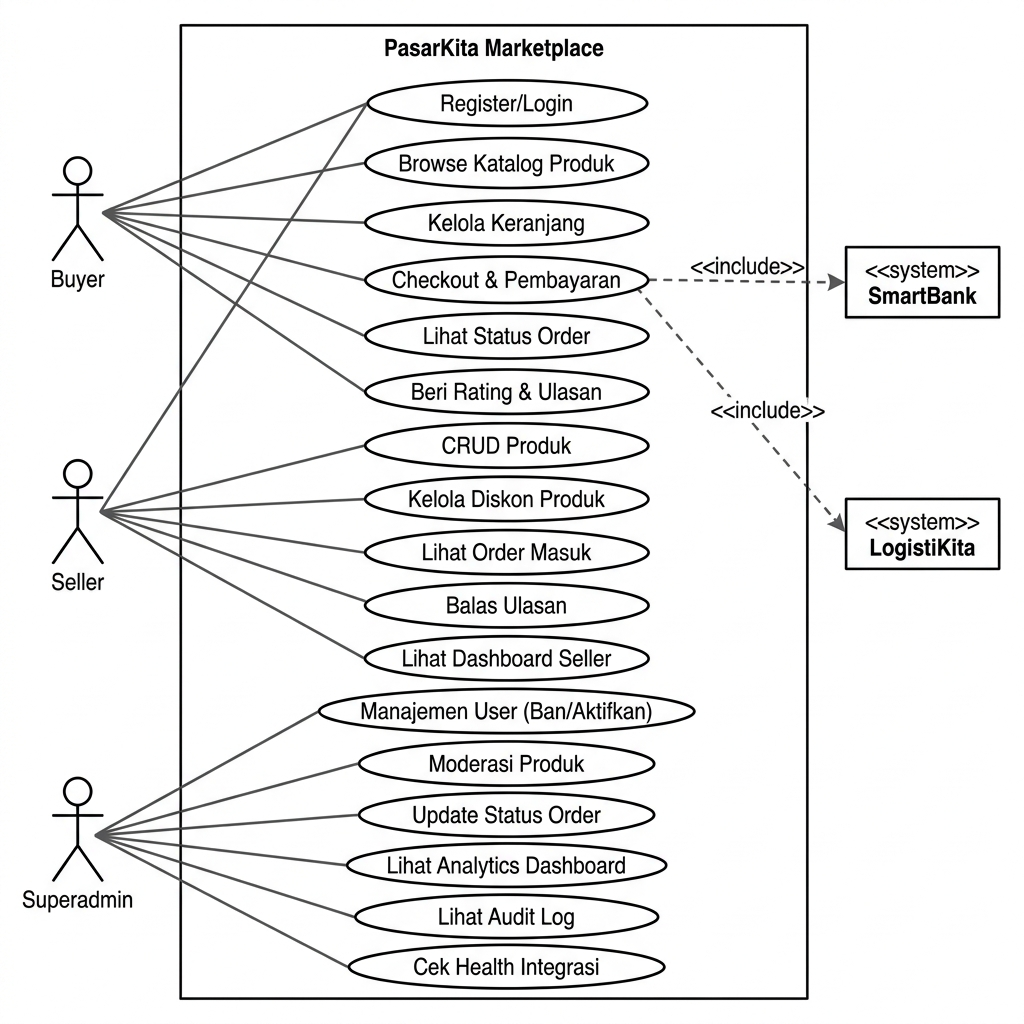
\includegraphics[width=\textwidth]{figures/usecase-diagram.png}
    \caption{Use Case Diagram Utama Sistem PasarKita}
    \label{fig:usecase-utama}
\end{figure}

\begin{longtable}{|L{2.5cm}|L{3cm}|L{5cm}|L{4cm}|}
    \caption{Workflow Operasional Utama Sistem PasarKita}
    \label{tab:workflow} \\
    \hline
    \textbf{Workflow} & \textbf{Trigger} & \textbf{Main Success Scenario}
        & \textbf{Failure / Control} \\
    \hline
    \endfirsthead
    \hline
    \textbf{Workflow} & \textbf{Trigger} & \textbf{Main Success Scenario}
        & \textbf{Failure / Control} \\
    \hline
    \endhead
    \hline
    \endfoot
    User Registration
        & \textit{User} membuka \texttt{/auth/register}.
        & Sistem memvalidasi \textit{input}, \textit{hash password}, simpan
          \textit{user}, inisiasi saldo Rp~50.000 ke SmartBank, kembalikan JWT.
        & Jika SmartBank tidak tersedia, \textit{user} tersimpan namun saldo
          belum terinisiasi; perlu \textit{retry} manual atau \textit{background
          job}. \\
    \hline
    Product Listing
        & \textit{Seller} membuka \texttt{/seller/products}.
        & \textit{Seller} membuat produk dengan \textit{form} valid; produk aktif
          dan tampil di katalog \textit{buyer}.
        & Validasi Zod gagal mengembalikan daftar \textit{field error} eksplisit;
          produk tidak tersimpan. \\
    \hline
    Checkout \& Payment
        & \textit{Buyer} menekan tombol ``Bayar'' di halaman \textit{checkout}.
        & \textit{Backend} validasi stok $\rightarrow$ kalkulasi \textit{fee}
          $\rightarrow$ buat \textit{order} pending $\rightarrow$
          \textit{payment request} ke SmartBank $\rightarrow$ \textit{update}
          \texttt{paid} $\rightarrow$ \textit{trigger} LogistiKita $\rightarrow$
          kembalikan konfirmasi.
        & Stok tidak cukup: 400 \texttt{INSUFFICIENT\_STOCK}. SmartBank gagal:
          402 \texttt{PAYMENT\_FAILED}, stok di-\textit{rollback}, \textit{order}
          \texttt{payment\_failed}. \\
    \hline
    Order Tracking
        & \textit{Buyer} membuka \texttt{/orders/:id}.
        & Sistem menampilkan status \textit{order} terkini, \texttt{tracking\_id},
          estimasi pengiriman, dan riwayat status.
        & Jika \texttt{tracking\_id} belum ada (\textit{shipping trigger} gagal),
          tampilkan status ``Menunggu Pengiriman'' dengan notifikasi admin. \\
    \hline
    Review Submission
        & \textit{Buyer} membuka detail \textit{order} dengan status
          \texttt{delivered}.
        & \textit{Buyer} mengisi \textit{rating} dan komentar; sistem memvalidasi
          status \textit{order}; \textit{rating} tersimpan; rata-rata
          \textit{rating} produk diperbarui.
        & \textit{Rating} ditolak jika \textit{order} belum \texttt{delivered}
          atau sudah pernah di-\textit{rating}; pesan \textit{error} eksplisit
          ditampilkan. \\
    \hline
    Admin User Ban
        & \textit{Superadmin} membuka \texttt{/admin/users}.
        & \textit{Superadmin} memasukkan alasan ban; sistem men-\textit{set}
          \texttt{is\_active = false}, menulis \texttt{admin\_audit\_logs}, dan
          mengembalikan status terbaru.
        & \textit{User} yang di-ban tidak dapat \textit{login}; token aktif
          \textit{user} tersebut diinvalidasi pada \textit{request} berikutnya. \\
    \hline
    Integration Health Check
        & \textit{Superadmin} membuka halaman status integrasi.
        & Sistem melakukan \textit{ping} ke API Gateway, SmartBank, dan
          LogistiKita; menampilkan status \texttt{online}/\texttt{offline} dan
          \texttt{response\_ms}.
        & Jika \textit{service} eksternal \textit{offline}, \textit{dashboard}
          tetap berjalan; status ditampilkan sebagai \texttt{offline} dengan pesan
          \textit{error} terakhir. \\
    \hline
    Analytics Pull
        & \textit{Superadmin} membuka \texttt{/admin/analytics}.
        & Sistem mengembalikan metrik agregat: total \textit{revenue},
          \textit{order count}, distribusi status, produk terlaris, dan
          \textit{revenue} per \textit{seller}.
        & Jika \textit{query timeout}, \textit{dashboard} menampilkan pesan
          \textit{error} parsial; data lain yang berhasil dimuat tetap
          ditampilkan. \\
    \hline
\end{longtable}

\clearpage

% ============================================================
% BAB 9
% ============================================================
\section{Risiko, Kontrol, dan Acceptance Criteria}
% ============================================================
% BAB 9 - RISIKO, KONTROL, DAN ACCEPTANCE CRITERIA
% ============================================================

Karena sistem berada di antara proses transaksi keuangan dan logistik dalam
ekosistem \textit{microservices}, risiko utama bukan hanya \textit{bug} UI,
tetapi juga inkonsistensi stok, \textit{double charge}, dan perubahan kontrak
API yang tidak kompatibel.

\begin{longtable}{|L{1cm}|L{3.5cm}|L{4.5cm}|L{5.5cm}|}
    \caption{Risiko, Kontrol, dan Acceptance Criteria}
    \label{tab:risiko} \\
    \hline
    \textbf{Risk ID} & \textbf{Risiko} & \textbf{Kontrol Wajib}
        & \textbf{Acceptance Criteria} \\
    \hline
    \endfirsthead
    \hline
    \textbf{Risk ID} & \textbf{Risiko} & \textbf{Kontrol Wajib}
        & \textbf{Acceptance Criteria} \\
    \hline
    \endhead
    \hline
    \endfoot
    R-01
        & \textit{Double order} akibat \textit{retry checkout}.
        & \textit{Idempotency key} wajib pada setiap \textit{checkout};
          \textit{backend} mendeteksi dan mengembalikan \textit{order existing}.
        & \textit{Checkout} duplikat dengan \textit{key} yang sama tidak membuat
          \textit{order} baru; \textit{response} mengembalikan \textit{order}
          pertama. \\
    \hline
    R-02
        & Stok berkurang meski pembayaran gagal.
        & Stok di-\textit{reserve} saat \textit{order} \texttt{pending};
          \textit{rollback} stok dilakukan segera setelah SmartBank mengembalikan
          \textit{failure}.
        & Setelah \textit{payment failure}, \texttt{stock} produk kembali ke
          nilai sebelum \textit{checkout}; \textit{order} berstatus
          \texttt{payment\_failed}. \\
    \hline
    R-03
        & \textit{Service} SmartBank atau LogistiKita tidak tersedia saat
          \textit{checkout}.
        & \textit{Failure handling} dengan \textit{timeout}, \textit{error
          response} bermakna, pencatatan di \texttt{integration\_logs};
          \textit{checkout} tidak menggantung tanpa batas.
        & \textit{Timeout} ke SmartBank menghasilkan 503
          \texttt{SERVICE\_UNAVAILABLE} dengan pesan yang dapat dimengerti
          \textit{buyer}; \textit{order} tidak terbuat. \\
    \hline
    R-04
        & Perubahan kontrak API memutus integrasi dengan \textit{service partner}.
        & \textit{Backward compatibility} wajib; \textit{field} baru bersifat
          \textit{additive}; perubahan \textit{breaking} didiskusikan lintas
          kelompok sebelum \textit{deploy}.
        & \textit{Service partner} dapat membaca \textit{response} API setelah
          \textit{update} tanpa perubahan kode di sisi mereka untuk \textit{field}
          yang sudah ada. \\
    \hline
    R-05
        & Akses tidak sah ke data \textit{user} atau \textit{order} lain.
        & \textit{Role-based middleware} memvalidasi kepemilikan \textit{resource};
          \textit{buyer} hanya melihat \textit{order} sendiri; \textit{seller}
          hanya kelola produk sendiri.
        & \textit{Request} akses ke \textit{resource} \textit{user} lain
          menghasilkan 403 \textit{Forbidden}; tidak ada data \textit{user} lain
          yang ter-\textit{expose}. \\
    \hline
    R-06
        & Harga produk berubah setelah \textit{order} dibuat, memengaruhi laporan.
        & \texttt{price\_at\_purchase} adalah \textit{snapshot} \textit{immutable}
          saat transaksi; kalkulasi \textit{revenue} menggunakan \textit{field} ini.
        & \textit{Update} harga produk tidak memengaruhi nilai \texttt{subtotal}
          pada \textit{order} yang sudah ada. \\
    \hline
    R-07
        & \textit{Superadmin} tidak dapat diaudit.
        & \texttt{admin\_audit\_logs} menulis setiap aksi sensitif dengan
          \texttt{before\_data} dan \texttt{after\_data}.
        & Setiap aksi ban \textit{user} dan \textit{update} status \textit{order}
          menghasilkan entri \textit{audit log} yang dapat ditelusuri oleh
          aktor. \\
    \hline
\end{longtable}

\clearpage

% ============================================================
% BAB 10
% ============================================================
\section{Matriks Ketertelusuran}
% ============================================================
% BAB 10 - MATRIKS KETERTELUSURAN
% ============================================================

\textit{Traceability matrix} menghubungkan \textit{objective} produk dengan
\textit{requirement} dan bukti verifikasi. Matriks ini membantu \textit{developer}
dan QA memastikan perubahan kode tetap menjaga tujuan sistem.

\begin{longtable}{|L{4cm}|L{3.5cm}|L{7cm}|}
    \caption{Matriks Ketertelusuran Requirement PasarKita}
    \label{tab:traceability} \\
    \hline
    \textbf{Objective} & \textbf{Requirement IDs} & \textbf{Evidence / Verification} \\
    \hline
    \endfirsthead
    \hline
    \textbf{Objective} & \textbf{Requirement IDs} & \textbf{Evidence / Verification} \\
    \hline
    \endhead
    \hline
    \endfoot
    \textit{User} dapat mendaftar dan \textit{login} dengan \textit{role} yang
    tepat.
        & FR-01, FR-02, FR-03, NFR-01, NFR-02
        & \textit{Test} register \textit{buyer}/\textit{seller}/\textit{superadmin};
          \textit{test} \textit{login} valid/invalid; \textit{test} token
          \textit{expired}. \\
    \hline
    \textit{Buyer} dapat menelusuri dan membeli produk UMKM.
        & FR-04, FR-05, FR-08, FR-09, FR-10, NFR-04
        & \textit{Test} katalog dengan filter; \textit{test} \textit{checkout}
          sukses; \textit{test} \textit{checkout} dengan stok habis; \textit{test}
          \textit{idempotency}. \\
    \hline
    \textit{Seller} dapat mengelola katalog produk secara mandiri.
        & FR-06, FR-07, FR-22, NFR-03, NFR-08
        & \textit{Test} CRUD produk \textit{seller}; \textit{test} akses ke produk
          \textit{seller} lain; \textit{test} diskon produk. \\
    \hline
    Transaksi keuangan terintegrasi dengan SmartBank via API Gateway.
        & FR-09, FR-10, FR-12, BR-01, BR-03, NFR-05, NFR-07
        & \textit{Test} \textit{checkout} sukses dan gagal; \textit{test} kalkulasi
          \textit{fee}; \textit{test} \textit{rate limiting}; simulasi SmartBank
          \textit{offline}. \\
    \hline
    Pengiriman terkoordinasi dengan LogistiKita.
        & FR-11, R-03, NFR-07
        & \textit{Test} \textit{trigger} pengiriman setelah \textit{payment} sukses;
          simulasi LogistiKita \textit{offline}; verifikasi \texttt{tracking\_id}
          tersimpan. \\
    \hline
    Admin dapat mengelola platform dan memantau \textit{analytics}.
        & FR-16, FR-19, FR-20, FR-21, NFR-09
        & \textit{Test} ban/aktifkan \textit{user}; \textit{test} \textit{update}
          status \textit{order}; \textit{test} \textit{analytics endpoint};
          verifikasi \textit{audit log}. \\
    \hline
    Sistem tetap tangguh saat \textit{dependency} eksternal gagal.
        & NFR-06, NFR-07, R-03, R-04
        & Matikan \textit{mock} SmartBank/LogistiKita; verifikasi
          \textit{error handling}; verifikasi \texttt{integration\_logs} tercatat. \\
    \hline
    Data transaksi terlindungi dan teraudit.
        & NFR-01, NFR-03, NFR-09, NFR-12, R-05, R-06
        & \textit{Test} akses lintas \textit{user}; verifikasi
          \texttt{password\_hash} tidak ter-\textit{expose}; verifikasi
          \textit{snapshot} harga \textit{immutable}. \\
    \hline
\end{longtable}

\clearpage

% ============================================================
% LAMPIRAN
% ============================================================
% ============================================================
% LAMPIRAN
% ============================================================

% ---- Lampiran A ----
\section*{LAMPIRAN A \\ GLOSARIUM}
\phantomsection
\addcontentsline{toc}{section}{LAMPIRAN A GLOSARIUM}
\refstepcounter{section}

\begin{longtable}{|L{4cm}|L{11cm}|}
    \caption{Glosarium Istilah SRS PasarKita}
    \label{tab:glosarium} \\
    \hline
    \textbf{Istilah} & \textbf{Definisi Operasional} \\
    \hline
    \endfirsthead
    \hline
    \textbf{Istilah} & \textbf{Definisi Operasional} \\
    \hline
    \endhead
    \hline
    \endfoot
    PasarKita
        & Platform \textit{marketplace} digital B2C untuk produk UMKM;
          \textit{Demand Generator} dalam ekosistem RPL 2. \\
    \hline
    Ekosistem UMKM RPL 2
        & Kumpulan \textit{microservices} antar kelompok yang saling terintegrasi:
          SmartBank, WarungPOS, SupplierHub, LogistiKita, UMKM Insight, dan API
          Gateway. \\
    \hline
    API Gateway
        & \textit{Service} Kelompok 7 yang bertindak sebagai \textit{routing layer},
          JWT \textit{validator} antar-\textit{service}, dan \textit{logging}
          inter-\textit{service}. \\
    \hline
    SmartBank
        & \textit{Service} Kelompok 1 sebagai \textit{core} keuangan; memproses
          pembayaran dan mengelola saldo \textit{user}. \\
    \hline
    LogistiKita
        & \textit{Service} Kelompok 5 yang mengelola pengiriman dan menghasilkan
          \texttt{tracking\_id}. \\
    \hline
    \textit{Demand Generator}
        & Peran PasarKita sebagai inisiator permintaan (\textit{buyer} melakukan
          \textit{checkout}) dalam ekosistem. \\
    \hline
    \textit{Idempotency Key}
        & UUID unik yang dikirimkan pada setiap \textit{checkout request} untuk
          mencegah pemrosesan duplikat. \\
    \hline
    \textit{Snapshot} Harga
        & Nilai \texttt{price\_at\_purchase} pada \texttt{order\_items} yang
          diambil saat transaksi dan tidak berubah meskipun harga produk
          diperbarui. \\
    \hline
    \textit{Soft Delete}
        & Penghapusan logis dengan mengubah \texttt{is\_active = false} tanpa
          menghapus \textit{record} dari \textit{database}. \\
    \hline
    \textit{Fee Marketplace}
        & Biaya platform sebesar 2\% dari subtotal \textit{order} yang dibebankan
          ke \textit{buyer} setiap transaksi. \\
    \hline
    \textit{Mock Server}
        & Implementasi lokal di \texttt{mock/} yang mensimulasikan SmartBank dan
          LogistiKita untuk keperluan \textit{development} tanpa bergantung pada
          \textit{service} nyata. \\
    \hline
    \textit{System of Record}
        & Sistem otoritatif untuk satu jenis data. PasarKita adalah
          \textit{system of record} untuk produk, \textit{order}, dan ulasan dalam
          ekosistemnya; SmartBank adalah \textit{system of record} untuk saldo dan
          transaksi keuangan. \\
    \hline
\end{longtable}

\clearpage

% ---- Lampiran B ----
\section*{LAMPIRAN B \\ REFERENSI INTERNAL}
\phantomsection
\addcontentsline{toc}{section}{LAMPIRAN B REFERENSI INTERNAL}
\refstepcounter{section}

\begin{longtable}{|L{6cm}|L{9cm}|}
    \caption{Referensi Internal Artefak Proyek PasarKita}
    \label{tab:referensi-internal} \\
    \hline
    \textbf{Artefak} & \textbf{Relevansi} \\
    \hline
    \endfirsthead
    \hline
    \textbf{Artefak} & \textbf{Relevansi} \\
    \hline
    \endhead
    \hline
    \endfoot
    \path{README.md}
        & Deskripsi umum aplikasi, arsitektur ekosistem, \textit{tech stack},
          API \textit{endpoints}, \textit{role} \& akses, dan aturan keuangan
          ekosistem. \\
    \hline
    \path{backend/database/schema/000_full_schema.sql}
        & Skema lengkap semua tabel Supabase PostgreSQL: \texttt{users},
          \texttt{products}, \texttt{orders}, \texttt{order\_items},
          \texttt{ratings}, \texttt{notifications}, \texttt{vouchers},
          \texttt{integration\_logs}, \texttt{admin\_audit\_logs}, dan lainnya. \\
    \hline
    \path{backend/src/modules/}
        & \textit{Business logic} per domain: auth, products, orders,
          \textit{checkout}, dan integrations. \\
    \hline
    \path{backend/src/middlewares/}
        & \textit{Middleware} auth (JWT validation), validate (Zod
          \textit{schema}), dan errorHandler (\textit{centralized error
          response}). \\
    \hline
    \path{backend/src/integrations/}
        & Adapter HTTP untuk SmartBank dan LogistiKita; konfigurasi
          \texttt{GATEWAY\_BASE\_URL} vs \textit{mock} URL. \\
    \hline
    \path{backend/src/utils/fee.js}
        & Implementasi kalkulasi \textit{fee marketplace} 2\%; digunakan oleh
          \textit{checkout module} dan \textit{fee simulation endpoint}. \\
    \hline
    \path{backend/vercel.json}
        & Konfigurasi \textit{routing} Vercel untuk \textit{backend serverless};
          memetakan semua \textit{path} ke \texttt{api/index.js}. \\
    \hline
    \path{frontend/store/}
        & Zustand \textit{store} untuk auth \textit{state} (\textit{user},
          \textit{token}, \textit{login}/\textit{logout}) dan \textit{cart state}
          (\textit{items}, add, remove, clear). \\
    \hline
    \path{mock/smartbank/} dan \path{mock/logistikita/}
        & Implementasi \textit{mock server} lokal; digunakan hanya saat
          \texttt{NODE\_ENV=development}. \\
    \hline
\end{longtable}

\clearpage

% ---- Lampiran C ----
\section*{LAMPIRAN C \\ CATATAN PERUBAHAN VERSI}
\phantomsection
\addcontentsline{toc}{section}{LAMPIRAN C CATATAN PERUBAHAN VERSI}
\refstepcounter{section}

\begin{longtable}{|L{1.5cm}|L{3.5cm}|L{10cm}|}
    \caption{Catatan Perubahan Versi Dokumen SRS}
    \label{tab:changelog} \\
    \hline
    \textbf{Versi} & \textbf{Tanggal} & \textbf{Keterangan} \\
    \hline
    \endfirsthead
    \hline
    \textbf{Versi} & \textbf{Tanggal} & \textbf{Keterangan} \\
    \hline
    \endhead
    \hline
    \endfoot
    1.0
        & [Tanggal]
        & \textit{Initial baseline} SRS; disusun dari README, skema
          \textit{database}, dan struktur kode aktif. Mencakup semua bagian:
          pendahuluan, gambaran produk, arsitektur, domain data, kebutuhan
          fungsional (FR-01 s/d FR-22), kebutuhan non-fungsional (NFR-01 s/d
          NFR-12), antarmuka eksternal, \textit{workflow} operasional, risiko, dan
          \textit{traceability matrix}. \\
    \hline
\end{longtable}

\clearpage

\end{document}
